% Created by tikzDevice version 0.12 on 2019-05-20 10:59:51
% !TEX encoding = UTF-8 Unicode
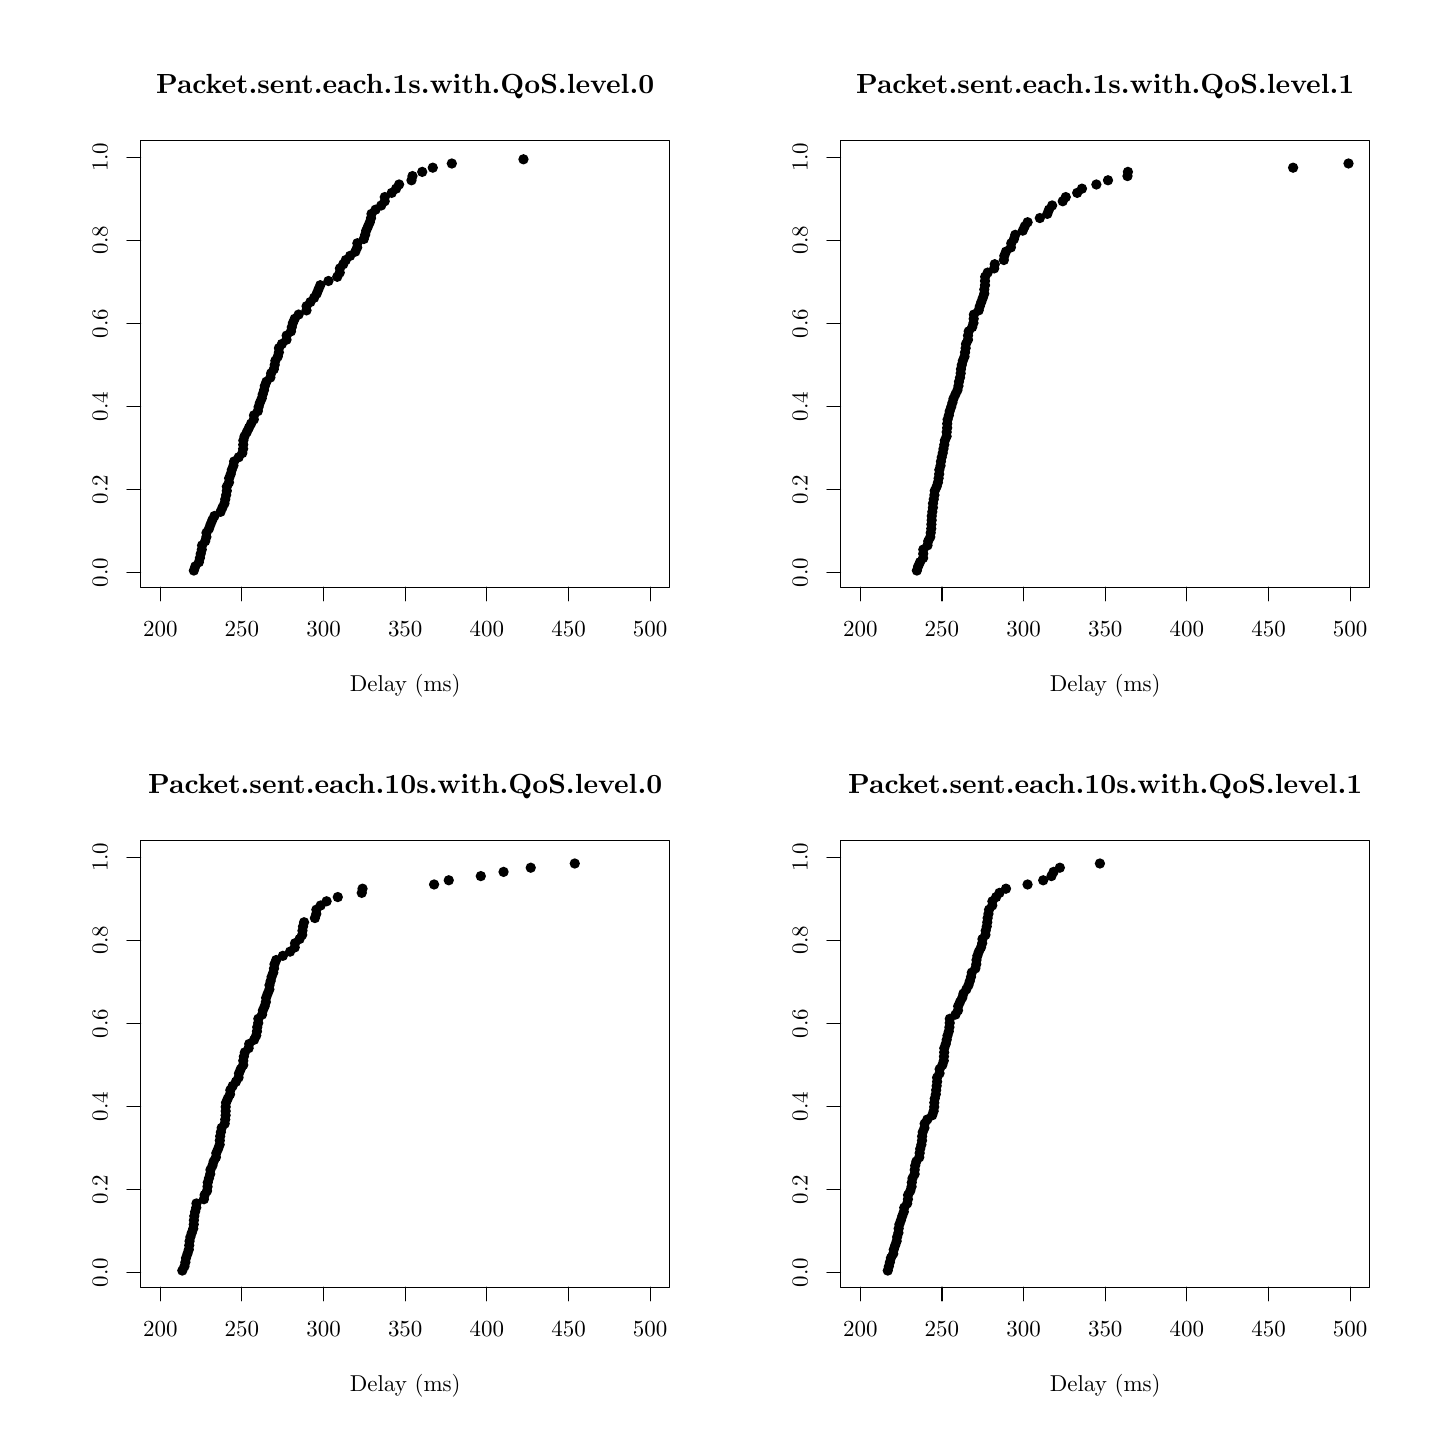
\begin{tikzpicture}[x=1pt,y=1pt]
\definecolor{fillColor}{RGB}{255,255,255}
\path[use as bounding box,fill=fillColor,fill opacity=0.00] (0,0) rectangle (505.89,505.89);
\begin{scope}
\path[clip] ( 40.84,303.74) rectangle (232.03,465.05);
\definecolor{fillColor}{RGB}{0,0,0}

\path[fill=fillColor] ( 60.05,309.72) circle (  1.87);

\path[fill=fillColor] ( 60.58,311.23) circle (  1.87);

\path[fill=fillColor] ( 61.87,312.75) circle (  1.87);

\path[fill=fillColor] ( 62.24,314.26) circle (  1.87);

\path[fill=fillColor] ( 62.53,315.78) circle (  1.87);

\path[fill=fillColor] ( 62.92,317.30) circle (  1.87);

\path[fill=fillColor] ( 63.02,318.81) circle (  1.87);

\path[fill=fillColor] ( 64.14,320.33) circle (  1.87);

\path[fill=fillColor] ( 64.58,321.85) circle (  1.87);

\path[fill=fillColor] ( 64.61,323.36) circle (  1.87);

\path[fill=fillColor] ( 65.54,324.88) circle (  1.87);

\path[fill=fillColor] ( 66.08,326.40) circle (  1.87);

\path[fill=fillColor] ( 66.70,327.91) circle (  1.87);

\path[fill=fillColor] ( 67.49,329.43) circle (  1.87);

\path[fill=fillColor] ( 69.70,330.94) circle (  1.87);

\path[fill=fillColor] ( 70.37,332.46) circle (  1.87);

\path[fill=fillColor] ( 71.11,333.98) circle (  1.87);

\path[fill=fillColor] ( 71.40,335.49) circle (  1.87);

\path[fill=fillColor] ( 71.72,337.01) circle (  1.87);

\path[fill=fillColor] ( 71.96,338.53) circle (  1.87);

\path[fill=fillColor] ( 71.97,340.04) circle (  1.87);

\path[fill=fillColor] ( 72.75,341.56) circle (  1.87);

\path[fill=fillColor] ( 72.79,343.08) circle (  1.87);

\path[fill=fillColor] ( 73.38,344.59) circle (  1.87);

\path[fill=fillColor] ( 73.76,346.11) circle (  1.87);

\path[fill=fillColor] ( 74.35,347.63) circle (  1.87);

\path[fill=fillColor] ( 74.60,349.14) circle (  1.87);

\path[fill=fillColor] ( 76.25,350.66) circle (  1.87);

\path[fill=fillColor] ( 77.56,352.17) circle (  1.87);

\path[fill=fillColor] ( 77.85,353.69) circle (  1.87);

\path[fill=fillColor] ( 77.88,355.21) circle (  1.87);

\path[fill=fillColor] ( 77.93,356.72) circle (  1.87);

\path[fill=fillColor] ( 78.37,358.24) circle (  1.87);

\path[fill=fillColor] ( 79.20,359.76) circle (  1.87);

\path[fill=fillColor] ( 79.94,361.27) circle (  1.87);

\path[fill=fillColor] ( 80.73,362.79) circle (  1.87);

\path[fill=fillColor] ( 81.72,364.31) circle (  1.87);

\path[fill=fillColor] ( 81.78,365.82) circle (  1.87);

\path[fill=fillColor] ( 83.17,367.34) circle (  1.87);

\path[fill=fillColor] ( 83.45,368.85) circle (  1.87);

\path[fill=fillColor] ( 83.92,370.37) circle (  1.87);

\path[fill=fillColor] ( 84.57,371.89) circle (  1.87);

\path[fill=fillColor] ( 84.93,373.40) circle (  1.87);

\path[fill=fillColor] ( 85.41,374.92) circle (  1.87);

\path[fill=fillColor] ( 85.70,376.44) circle (  1.87);

\path[fill=fillColor] ( 86.27,377.95) circle (  1.87);

\path[fill=fillColor] ( 87.69,379.47) circle (  1.87);

\path[fill=fillColor] ( 87.96,380.99) circle (  1.87);

\path[fill=fillColor] ( 88.95,382.50) circle (  1.87);

\path[fill=fillColor] ( 89.26,384.02) circle (  1.87);

\path[fill=fillColor] ( 89.51,385.53) circle (  1.87);

\path[fill=fillColor] ( 90.37,387.05) circle (  1.87);

\path[fill=fillColor] ( 90.78,388.57) circle (  1.87);

\path[fill=fillColor] ( 90.79,390.08) circle (  1.87);

\path[fill=fillColor] ( 91.87,391.60) circle (  1.87);

\path[fill=fillColor] ( 93.53,393.12) circle (  1.87);

\path[fill=fillColor] ( 93.58,394.63) circle (  1.87);

\path[fill=fillColor] ( 95.14,396.15) circle (  1.87);

\path[fill=fillColor] ( 95.44,397.67) circle (  1.87);

\path[fill=fillColor] ( 95.84,399.18) circle (  1.87);

\path[fill=fillColor] ( 96.50,400.70) circle (  1.87);

\path[fill=fillColor] ( 97.91,402.22) circle (  1.87);

\path[fill=fillColor] (100.75,403.73) circle (  1.87);

\path[fill=fillColor] (100.78,405.25) circle (  1.87);

\path[fill=fillColor] (102.18,406.76) circle (  1.87);

\path[fill=fillColor] (103.50,408.28) circle (  1.87);

\path[fill=fillColor] (104.46,409.80) circle (  1.87);

\path[fill=fillColor] (105.07,411.31) circle (  1.87);

\path[fill=fillColor] (105.73,412.83) circle (  1.87);

\path[fill=fillColor] (108.69,414.35) circle (  1.87);

\path[fill=fillColor] (111.87,415.86) circle (  1.87);

\path[fill=fillColor] (112.77,417.38) circle (  1.87);

\path[fill=fillColor] (112.83,418.90) circle (  1.87);

\path[fill=fillColor] (114.04,420.41) circle (  1.87);

\path[fill=fillColor] (114.96,421.93) circle (  1.87);

\path[fill=fillColor] (116.52,423.44) circle (  1.87);

\path[fill=fillColor] (118.40,424.96) circle (  1.87);

\path[fill=fillColor] (119.07,426.48) circle (  1.87);

\path[fill=fillColor] (119.13,427.99) circle (  1.87);

\path[fill=fillColor] (121.45,429.51) circle (  1.87);

\path[fill=fillColor] (121.95,431.03) circle (  1.87);

\path[fill=fillColor] (122.32,432.54) circle (  1.87);

\path[fill=fillColor] (122.98,434.06) circle (  1.87);

\path[fill=fillColor] (123.63,435.58) circle (  1.87);

\path[fill=fillColor] (124.07,437.09) circle (  1.87);

\path[fill=fillColor] (124.25,438.61) circle (  1.87);

\path[fill=fillColor] (125.70,440.12) circle (  1.87);

\path[fill=fillColor] (127.75,441.64) circle (  1.87);

\path[fill=fillColor] (129.01,443.16) circle (  1.87);

\path[fill=fillColor] (129.04,444.67) circle (  1.87);

\path[fill=fillColor] (131.55,446.19) circle (  1.87);

\path[fill=fillColor] (133.13,447.71) circle (  1.87);

\path[fill=fillColor] (134.21,449.22) circle (  1.87);

\path[fill=fillColor] (138.69,450.74) circle (  1.87);

\path[fill=fillColor] (139.05,452.26) circle (  1.87);

\path[fill=fillColor] (142.57,453.77) circle (  1.87);

\path[fill=fillColor] (146.38,455.29) circle (  1.87);

\path[fill=fillColor] (153.26,456.80) circle (  1.87);

\path[fill=fillColor] (179.15,458.32) circle (  1.87);
\end{scope}
\begin{scope}
\path[clip] (  0.00,  0.00) rectangle (505.89,505.89);
\definecolor{drawColor}{RGB}{0,0,0}

\path[draw=drawColor,line width= 0.4pt,line join=round,line cap=round] ( 47.92,303.74) -- (224.95,303.74);

\path[draw=drawColor,line width= 0.4pt,line join=round,line cap=round] ( 47.92,303.74) -- ( 47.92,298.76);

\path[draw=drawColor,line width= 0.4pt,line join=round,line cap=round] ( 77.42,303.74) -- ( 77.42,298.76);

\path[draw=drawColor,line width= 0.4pt,line join=round,line cap=round] (106.93,303.74) -- (106.93,298.76);

\path[draw=drawColor,line width= 0.4pt,line join=round,line cap=round] (136.43,303.74) -- (136.43,298.76);

\path[draw=drawColor,line width= 0.4pt,line join=round,line cap=round] (165.94,303.74) -- (165.94,298.76);

\path[draw=drawColor,line width= 0.4pt,line join=round,line cap=round] (195.44,303.74) -- (195.44,298.76);

\path[draw=drawColor,line width= 0.4pt,line join=round,line cap=round] (224.95,303.74) -- (224.95,298.76);

\node[text=drawColor,anchor=base,inner sep=0pt, outer sep=0pt, scale=  0.83] at ( 47.92,285.81) {200};

\node[text=drawColor,anchor=base,inner sep=0pt, outer sep=0pt, scale=  0.83] at ( 77.42,285.81) {250};

\node[text=drawColor,anchor=base,inner sep=0pt, outer sep=0pt, scale=  0.83] at (106.93,285.81) {300};

\node[text=drawColor,anchor=base,inner sep=0pt, outer sep=0pt, scale=  0.83] at (136.43,285.81) {350};

\node[text=drawColor,anchor=base,inner sep=0pt, outer sep=0pt, scale=  0.83] at (165.94,285.81) {400};

\node[text=drawColor,anchor=base,inner sep=0pt, outer sep=0pt, scale=  0.83] at (195.44,285.81) {450};

\node[text=drawColor,anchor=base,inner sep=0pt, outer sep=0pt, scale=  0.83] at (224.95,285.81) {500};

\path[draw=drawColor,line width= 0.4pt,line join=round,line cap=round] ( 40.84,308.96) -- ( 40.84,459.08);

\path[draw=drawColor,line width= 0.4pt,line join=round,line cap=round] ( 40.84,308.96) -- ( 35.86,308.96);

\path[draw=drawColor,line width= 0.4pt,line join=round,line cap=round] ( 40.84,338.98) -- ( 35.86,338.98);

\path[draw=drawColor,line width= 0.4pt,line join=round,line cap=round] ( 40.84,369.01) -- ( 35.86,369.01);

\path[draw=drawColor,line width= 0.4pt,line join=round,line cap=round] ( 40.84,399.03) -- ( 35.86,399.03);

\path[draw=drawColor,line width= 0.4pt,line join=round,line cap=round] ( 40.84,429.06) -- ( 35.86,429.06);

\path[draw=drawColor,line width= 0.4pt,line join=round,line cap=round] ( 40.84,459.08) -- ( 35.86,459.08);

\node[text=drawColor,rotate= 90.00,anchor=base,inner sep=0pt, outer sep=0pt, scale=  0.83] at ( 28.88,308.96) {0.0};

\node[text=drawColor,rotate= 90.00,anchor=base,inner sep=0pt, outer sep=0pt, scale=  0.83] at ( 28.88,338.98) {0.2};

\node[text=drawColor,rotate= 90.00,anchor=base,inner sep=0pt, outer sep=0pt, scale=  0.83] at ( 28.88,369.01) {0.4};

\node[text=drawColor,rotate= 90.00,anchor=base,inner sep=0pt, outer sep=0pt, scale=  0.83] at ( 28.88,399.03) {0.6};

\node[text=drawColor,rotate= 90.00,anchor=base,inner sep=0pt, outer sep=0pt, scale=  0.83] at ( 28.88,429.06) {0.8};

\node[text=drawColor,rotate= 90.00,anchor=base,inner sep=0pt, outer sep=0pt, scale=  0.83] at ( 28.88,459.08) {1.0};

\path[draw=drawColor,line width= 0.4pt,line join=round,line cap=round] ( 40.84,303.74) --
	(232.03,303.74) --
	(232.03,465.05) --
	( 40.84,465.05) --
	( 40.84,303.74);
\end{scope}
\begin{scope}
\path[clip] (  0.00,252.94) rectangle (252.94,505.89);
\definecolor{drawColor}{RGB}{0,0,0}

\node[text=drawColor,anchor=base,inner sep=0pt, outer sep=0pt, scale=  1.00] at (136.43,482.04) {\bfseries Packet.sent.each.1s.with.QoS.level.0};

\node[text=drawColor,anchor=base,inner sep=0pt, outer sep=0pt, scale=  0.83] at (136.43,265.89) {Delay (ms)};
\end{scope}
\begin{scope}
\path[clip] (293.78,303.74) rectangle (484.97,465.05);
\definecolor{fillColor}{RGB}{0,0,0}

\path[fill=fillColor] (321.31,309.72) circle (  1.87);

\path[fill=fillColor] (321.77,311.23) circle (  1.87);

\path[fill=fillColor] (322.45,312.75) circle (  1.87);

\path[fill=fillColor] (323.56,314.26) circle (  1.87);

\path[fill=fillColor] (323.60,315.78) circle (  1.87);

\path[fill=fillColor] (323.63,317.30) circle (  1.87);

\path[fill=fillColor] (325.15,318.81) circle (  1.87);

\path[fill=fillColor] (325.40,320.33) circle (  1.87);

\path[fill=fillColor] (326.15,321.85) circle (  1.87);

\path[fill=fillColor] (326.31,323.36) circle (  1.87);

\path[fill=fillColor] (326.51,324.88) circle (  1.87);

\path[fill=fillColor] (326.55,326.40) circle (  1.87);

\path[fill=fillColor] (326.66,327.91) circle (  1.87);

\path[fill=fillColor] (326.69,329.43) circle (  1.87);

\path[fill=fillColor] (326.89,330.94) circle (  1.87);

\path[fill=fillColor] (327.10,332.46) circle (  1.87);

\path[fill=fillColor] (327.14,333.98) circle (  1.87);

\path[fill=fillColor] (327.41,335.49) circle (  1.87);

\path[fill=fillColor] (327.65,337.01) circle (  1.87);

\path[fill=fillColor] (327.77,338.53) circle (  1.87);

\path[fill=fillColor] (328.45,340.04) circle (  1.87);

\path[fill=fillColor] (328.92,341.56) circle (  1.87);

\path[fill=fillColor] (329.17,343.08) circle (  1.87);

\path[fill=fillColor] (329.37,344.59) circle (  1.87);

\path[fill=fillColor] (329.43,346.11) circle (  1.87);

\path[fill=fillColor] (329.87,347.63) circle (  1.87);

\path[fill=fillColor] (330.00,349.14) circle (  1.87);

\path[fill=fillColor] (330.29,350.66) circle (  1.87);

\path[fill=fillColor] (330.66,352.17) circle (  1.87);

\path[fill=fillColor] (330.92,353.69) circle (  1.87);

\path[fill=fillColor] (331.22,355.21) circle (  1.87);

\path[fill=fillColor] (331.43,356.72) circle (  1.87);

\path[fill=fillColor] (332.06,358.24) circle (  1.87);

\path[fill=fillColor] (332.08,359.76) circle (  1.87);

\path[fill=fillColor] (332.25,361.27) circle (  1.87);

\path[fill=fillColor] (332.27,362.79) circle (  1.87);

\path[fill=fillColor] (332.42,364.31) circle (  1.87);

\path[fill=fillColor] (332.87,365.82) circle (  1.87);

\path[fill=fillColor] (333.18,367.34) circle (  1.87);

\path[fill=fillColor] (333.71,368.85) circle (  1.87);

\path[fill=fillColor] (334.15,370.37) circle (  1.87);

\path[fill=fillColor] (334.56,371.89) circle (  1.87);

\path[fill=fillColor] (335.24,373.40) circle (  1.87);

\path[fill=fillColor] (335.97,374.92) circle (  1.87);

\path[fill=fillColor] (336.34,376.44) circle (  1.87);

\path[fill=fillColor] (336.53,377.95) circle (  1.87);

\path[fill=fillColor] (336.91,379.47) circle (  1.87);

\path[fill=fillColor] (337.14,380.99) circle (  1.87);

\path[fill=fillColor] (337.24,382.50) circle (  1.87);

\path[fill=fillColor] (337.54,384.02) circle (  1.87);

\path[fill=fillColor] (337.92,385.53) circle (  1.87);

\path[fill=fillColor] (338.53,387.05) circle (  1.87);

\path[fill=fillColor] (338.72,388.57) circle (  1.87);

\path[fill=fillColor] (338.93,390.08) circle (  1.87);

\path[fill=fillColor] (339.06,391.60) circle (  1.87);

\path[fill=fillColor] (339.78,393.12) circle (  1.87);

\path[fill=fillColor] (339.78,394.63) circle (  1.87);

\path[fill=fillColor] (340.04,396.15) circle (  1.87);

\path[fill=fillColor] (341.28,397.67) circle (  1.87);

\path[fill=fillColor] (341.76,399.18) circle (  1.87);

\path[fill=fillColor] (341.84,400.70) circle (  1.87);

\path[fill=fillColor] (341.92,402.22) circle (  1.87);

\path[fill=fillColor] (343.64,403.73) circle (  1.87);

\path[fill=fillColor] (344.06,405.25) circle (  1.87);

\path[fill=fillColor] (344.59,406.76) circle (  1.87);

\path[fill=fillColor] (345.15,408.28) circle (  1.87);

\path[fill=fillColor] (345.67,409.80) circle (  1.87);

\path[fill=fillColor] (345.67,411.31) circle (  1.87);

\path[fill=fillColor] (345.93,412.83) circle (  1.87);

\path[fill=fillColor] (345.93,414.35) circle (  1.87);

\path[fill=fillColor] (345.98,415.86) circle (  1.87);

\path[fill=fillColor] (346.89,417.38) circle (  1.87);

\path[fill=fillColor] (349.25,418.90) circle (  1.87);

\path[fill=fillColor] (349.45,420.41) circle (  1.87);

\path[fill=fillColor] (352.74,421.93) circle (  1.87);

\path[fill=fillColor] (352.91,423.44) circle (  1.87);

\path[fill=fillColor] (353.50,424.96) circle (  1.87);

\path[fill=fillColor] (355.28,426.48) circle (  1.87);

\path[fill=fillColor] (355.42,427.99) circle (  1.87);

\path[fill=fillColor] (356.39,429.51) circle (  1.87);

\path[fill=fillColor] (356.86,431.03) circle (  1.87);

\path[fill=fillColor] (359.58,432.54) circle (  1.87);

\path[fill=fillColor] (360.28,434.06) circle (  1.87);

\path[fill=fillColor] (361.32,435.58) circle (  1.87);

\path[fill=fillColor] (365.74,437.09) circle (  1.87);

\path[fill=fillColor] (368.46,438.61) circle (  1.87);

\path[fill=fillColor] (369.05,440.12) circle (  1.87);

\path[fill=fillColor] (370.19,441.64) circle (  1.87);

\path[fill=fillColor] (374.01,443.16) circle (  1.87);

\path[fill=fillColor] (375.11,444.67) circle (  1.87);

\path[fill=fillColor] (379.24,446.19) circle (  1.87);

\path[fill=fillColor] (380.96,447.71) circle (  1.87);

\path[fill=fillColor] (386.17,449.22) circle (  1.87);

\path[fill=fillColor] (390.37,450.74) circle (  1.87);

\path[fill=fillColor] (397.41,452.26) circle (  1.87);

\path[fill=fillColor] (397.57,453.77) circle (  1.87);

\path[fill=fillColor] (457.26,455.29) circle (  1.87);

\path[fill=fillColor] (477.28,456.81) circle (  1.87);

\path[fill=fillColor] (488.03,458.32) circle (  1.87);
\end{scope}
\begin{scope}
\path[clip] (  0.00,  0.00) rectangle (505.89,505.89);
\definecolor{drawColor}{RGB}{0,0,0}

\path[draw=drawColor,line width= 0.4pt,line join=round,line cap=round] (300.86,303.74) -- (477.89,303.74);

\path[draw=drawColor,line width= 0.4pt,line join=round,line cap=round] (300.86,303.74) -- (300.86,298.76);

\path[draw=drawColor,line width= 0.4pt,line join=round,line cap=round] (330.37,303.74) -- (330.37,298.76);

\path[draw=drawColor,line width= 0.4pt,line join=round,line cap=round] (359.87,303.74) -- (359.87,298.76);

\path[draw=drawColor,line width= 0.4pt,line join=round,line cap=round] (389.38,303.74) -- (389.38,298.76);

\path[draw=drawColor,line width= 0.4pt,line join=round,line cap=round] (418.88,303.74) -- (418.88,298.76);

\path[draw=drawColor,line width= 0.4pt,line join=round,line cap=round] (448.39,303.74) -- (448.39,298.76);

\path[draw=drawColor,line width= 0.4pt,line join=round,line cap=round] (477.89,303.74) -- (477.89,298.76);

\node[text=drawColor,anchor=base,inner sep=0pt, outer sep=0pt, scale=  0.83] at (300.86,285.81) {200};

\node[text=drawColor,anchor=base,inner sep=0pt, outer sep=0pt, scale=  0.83] at (330.37,285.81) {250};

\node[text=drawColor,anchor=base,inner sep=0pt, outer sep=0pt, scale=  0.83] at (359.87,285.81) {300};

\node[text=drawColor,anchor=base,inner sep=0pt, outer sep=0pt, scale=  0.83] at (389.38,285.81) {350};

\node[text=drawColor,anchor=base,inner sep=0pt, outer sep=0pt, scale=  0.83] at (418.88,285.81) {400};

\node[text=drawColor,anchor=base,inner sep=0pt, outer sep=0pt, scale=  0.83] at (448.39,285.81) {450};

\node[text=drawColor,anchor=base,inner sep=0pt, outer sep=0pt, scale=  0.83] at (477.89,285.81) {500};

\path[draw=drawColor,line width= 0.4pt,line join=round,line cap=round] (293.78,308.96) -- (293.78,459.08);

\path[draw=drawColor,line width= 0.4pt,line join=round,line cap=round] (293.78,308.96) -- (288.80,308.96);

\path[draw=drawColor,line width= 0.4pt,line join=round,line cap=round] (293.78,338.98) -- (288.80,338.98);

\path[draw=drawColor,line width= 0.4pt,line join=round,line cap=round] (293.78,369.01) -- (288.80,369.01);

\path[draw=drawColor,line width= 0.4pt,line join=round,line cap=round] (293.78,399.03) -- (288.80,399.03);

\path[draw=drawColor,line width= 0.4pt,line join=round,line cap=round] (293.78,429.06) -- (288.80,429.06);

\path[draw=drawColor,line width= 0.4pt,line join=round,line cap=round] (293.78,459.08) -- (288.80,459.08);

\node[text=drawColor,rotate= 90.00,anchor=base,inner sep=0pt, outer sep=0pt, scale=  0.83] at (281.83,308.96) {0.0};

\node[text=drawColor,rotate= 90.00,anchor=base,inner sep=0pt, outer sep=0pt, scale=  0.83] at (281.83,338.98) {0.2};

\node[text=drawColor,rotate= 90.00,anchor=base,inner sep=0pt, outer sep=0pt, scale=  0.83] at (281.83,369.01) {0.4};

\node[text=drawColor,rotate= 90.00,anchor=base,inner sep=0pt, outer sep=0pt, scale=  0.83] at (281.83,399.03) {0.6};

\node[text=drawColor,rotate= 90.00,anchor=base,inner sep=0pt, outer sep=0pt, scale=  0.83] at (281.83,429.06) {0.8};

\node[text=drawColor,rotate= 90.00,anchor=base,inner sep=0pt, outer sep=0pt, scale=  0.83] at (281.83,459.08) {1.0};

\path[draw=drawColor,line width= 0.4pt,line join=round,line cap=round] (293.78,303.74) --
	(484.97,303.74) --
	(484.97,465.05) --
	(293.78,465.05) --
	(293.78,303.74);
\end{scope}
\begin{scope}
\path[clip] (252.94,252.94) rectangle (505.89,505.89);
\definecolor{drawColor}{RGB}{0,0,0}

\node[text=drawColor,anchor=base,inner sep=0pt, outer sep=0pt, scale=  1.00] at (389.38,482.04) {\bfseries Packet.sent.each.1s.with.QoS.level.1};

\node[text=drawColor,anchor=base,inner sep=0pt, outer sep=0pt, scale=  0.83] at (389.38,265.89) {Delay (ms)};
\end{scope}
\begin{scope}
\path[clip] ( 40.84, 50.80) rectangle (232.03,212.11);
\definecolor{fillColor}{RGB}{0,0,0}

\path[fill=fillColor] ( 55.88, 56.77) circle (  1.87);

\path[fill=fillColor] ( 56.65, 58.29) circle (  1.87);

\path[fill=fillColor] ( 56.99, 59.80) circle (  1.87);

\path[fill=fillColor] ( 57.22, 61.32) circle (  1.87);

\path[fill=fillColor] ( 57.74, 62.84) circle (  1.87);

\path[fill=fillColor] ( 58.23, 64.35) circle (  1.87);

\path[fill=fillColor] ( 58.38, 65.87) circle (  1.87);

\path[fill=fillColor] ( 58.50, 67.39) circle (  1.87);

\path[fill=fillColor] ( 58.80, 68.90) circle (  1.87);

\path[fill=fillColor] ( 59.30, 70.42) circle (  1.87);

\path[fill=fillColor] ( 59.83, 71.93) circle (  1.87);

\path[fill=fillColor] ( 60.02, 73.45) circle (  1.87);

\path[fill=fillColor] ( 60.07, 74.97) circle (  1.87);

\path[fill=fillColor] ( 60.21, 76.48) circle (  1.87);

\path[fill=fillColor] ( 60.50, 78.00) circle (  1.87);

\path[fill=fillColor] ( 60.91, 79.52) circle (  1.87);

\path[fill=fillColor] ( 60.99, 81.03) circle (  1.87);

\path[fill=fillColor] ( 63.68, 82.55) circle (  1.87);

\path[fill=fillColor] ( 63.94, 84.07) circle (  1.87);

\path[fill=fillColor] ( 64.82, 85.58) circle (  1.87);

\path[fill=fillColor] ( 65.00, 87.10) circle (  1.87);

\path[fill=fillColor] ( 65.08, 88.61) circle (  1.87);

\path[fill=fillColor] ( 65.51, 90.13) circle (  1.87);

\path[fill=fillColor] ( 65.96, 91.65) circle (  1.87);

\path[fill=fillColor] ( 66.04, 93.16) circle (  1.87);

\path[fill=fillColor] ( 66.76, 94.68) circle (  1.87);

\path[fill=fillColor] ( 67.21, 96.20) circle (  1.87);

\path[fill=fillColor] ( 68.02, 97.71) circle (  1.87);

\path[fill=fillColor] ( 68.16, 99.23) circle (  1.87);

\path[fill=fillColor] ( 68.82,100.75) circle (  1.87);

\path[fill=fillColor] ( 69.38,102.26) circle (  1.87);

\path[fill=fillColor] ( 69.43,103.78) circle (  1.87);

\path[fill=fillColor] ( 69.56,105.30) circle (  1.87);

\path[fill=fillColor] ( 69.82,106.81) circle (  1.87);

\path[fill=fillColor] ( 70.10,108.33) circle (  1.87);

\path[fill=fillColor] ( 71.19,109.84) circle (  1.87);

\path[fill=fillColor] ( 71.38,111.36) circle (  1.87);

\path[fill=fillColor] ( 71.54,112.88) circle (  1.87);

\path[fill=fillColor] ( 71.55,114.39) circle (  1.87);

\path[fill=fillColor] ( 71.56,115.91) circle (  1.87);

\path[fill=fillColor] ( 71.67,117.43) circle (  1.87);

\path[fill=fillColor] ( 72.32,118.94) circle (  1.87);

\path[fill=fillColor] ( 73.12,120.46) circle (  1.87);

\path[fill=fillColor] ( 73.23,121.98) circle (  1.87);

\path[fill=fillColor] ( 74.08,123.49) circle (  1.87);

\path[fill=fillColor] ( 75.26,125.01) circle (  1.87);

\path[fill=fillColor] ( 76.20,126.52) circle (  1.87);

\path[fill=fillColor] ( 76.36,128.04) circle (  1.87);

\path[fill=fillColor] ( 76.99,129.56) circle (  1.87);

\path[fill=fillColor] ( 77.90,131.07) circle (  1.87);

\path[fill=fillColor] ( 77.90,132.59) circle (  1.87);

\path[fill=fillColor] ( 78.12,134.11) circle (  1.87);

\path[fill=fillColor] ( 78.48,135.62) circle (  1.87);

\path[fill=fillColor] ( 79.84,137.14) circle (  1.87);

\path[fill=fillColor] ( 80.05,138.66) circle (  1.87);

\path[fill=fillColor] ( 81.82,140.17) circle (  1.87);

\path[fill=fillColor] ( 82.58,141.69) circle (  1.87);

\path[fill=fillColor] ( 82.85,143.21) circle (  1.87);

\path[fill=fillColor] ( 82.95,144.72) circle (  1.87);

\path[fill=fillColor] ( 83.31,146.24) circle (  1.87);

\path[fill=fillColor] ( 83.35,147.75) circle (  1.87);

\path[fill=fillColor] ( 84.70,149.27) circle (  1.87);

\path[fill=fillColor] ( 84.99,150.79) circle (  1.87);

\path[fill=fillColor] ( 85.64,152.30) circle (  1.87);

\path[fill=fillColor] ( 86.07,153.82) circle (  1.87);

\path[fill=fillColor] ( 86.16,155.34) circle (  1.87);

\path[fill=fillColor] ( 86.72,156.85) circle (  1.87);

\path[fill=fillColor] ( 87.34,158.37) circle (  1.87);

\path[fill=fillColor] ( 87.38,159.89) circle (  1.87);

\path[fill=fillColor] ( 87.80,161.40) circle (  1.87);

\path[fill=fillColor] ( 88.15,162.92) circle (  1.87);

\path[fill=fillColor] ( 88.74,164.43) circle (  1.87);

\path[fill=fillColor] ( 89.02,165.95) circle (  1.87);

\path[fill=fillColor] ( 89.19,167.47) circle (  1.87);

\path[fill=fillColor] ( 89.80,168.98) circle (  1.87);

\path[fill=fillColor] ( 92.21,170.50) circle (  1.87);

\path[fill=fillColor] ( 94.82,172.02) circle (  1.87);

\path[fill=fillColor] ( 96.50,173.53) circle (  1.87);

\path[fill=fillColor] ( 96.61,175.05) circle (  1.87);

\path[fill=fillColor] ( 98.25,176.57) circle (  1.87);

\path[fill=fillColor] ( 99.20,178.08) circle (  1.87);

\path[fill=fillColor] ( 99.29,179.60) circle (  1.87);

\path[fill=fillColor] ( 99.50,181.12) circle (  1.87);

\path[fill=fillColor] ( 99.88,182.63) circle (  1.87);

\path[fill=fillColor] (103.79,184.15) circle (  1.87);

\path[fill=fillColor] (104.29,185.66) circle (  1.87);

\path[fill=fillColor] (104.32,187.18) circle (  1.87);

\path[fill=fillColor] (105.87,188.70) circle (  1.87);

\path[fill=fillColor] (108.02,190.21) circle (  1.87);

\path[fill=fillColor] (112.06,191.73) circle (  1.87);

\path[fill=fillColor] (120.72,193.25) circle (  1.87);

\path[fill=fillColor] (121.00,194.76) circle (  1.87);

\path[fill=fillColor] (146.86,196.28) circle (  1.87);

\path[fill=fillColor] (152.16,197.80) circle (  1.87);

\path[fill=fillColor] (163.74,199.31) circle (  1.87);

\path[fill=fillColor] (171.96,200.83) circle (  1.87);

\path[fill=fillColor] (181.78,202.34) circle (  1.87);

\path[fill=fillColor] (197.69,203.86) circle (  1.87);

\path[fill=fillColor] (266.83,205.38) circle (  1.87);
\end{scope}
\begin{scope}
\path[clip] (  0.00,  0.00) rectangle (505.89,505.89);
\definecolor{drawColor}{RGB}{0,0,0}

\path[draw=drawColor,line width= 0.4pt,line join=round,line cap=round] ( 47.92, 50.80) -- (224.95, 50.80);

\path[draw=drawColor,line width= 0.4pt,line join=round,line cap=round] ( 47.92, 50.80) -- ( 47.92, 45.82);

\path[draw=drawColor,line width= 0.4pt,line join=round,line cap=round] ( 77.42, 50.80) -- ( 77.42, 45.82);

\path[draw=drawColor,line width= 0.4pt,line join=round,line cap=round] (106.93, 50.80) -- (106.93, 45.82);

\path[draw=drawColor,line width= 0.4pt,line join=round,line cap=round] (136.43, 50.80) -- (136.43, 45.82);

\path[draw=drawColor,line width= 0.4pt,line join=round,line cap=round] (165.94, 50.80) -- (165.94, 45.82);

\path[draw=drawColor,line width= 0.4pt,line join=round,line cap=round] (195.44, 50.80) -- (195.44, 45.82);

\path[draw=drawColor,line width= 0.4pt,line join=round,line cap=round] (224.95, 50.80) -- (224.95, 45.82);

\node[text=drawColor,anchor=base,inner sep=0pt, outer sep=0pt, scale=  0.83] at ( 47.92, 32.87) {200};

\node[text=drawColor,anchor=base,inner sep=0pt, outer sep=0pt, scale=  0.83] at ( 77.42, 32.87) {250};

\node[text=drawColor,anchor=base,inner sep=0pt, outer sep=0pt, scale=  0.83] at (106.93, 32.87) {300};

\node[text=drawColor,anchor=base,inner sep=0pt, outer sep=0pt, scale=  0.83] at (136.43, 32.87) {350};

\node[text=drawColor,anchor=base,inner sep=0pt, outer sep=0pt, scale=  0.83] at (165.94, 32.87) {400};

\node[text=drawColor,anchor=base,inner sep=0pt, outer sep=0pt, scale=  0.83] at (195.44, 32.87) {450};

\node[text=drawColor,anchor=base,inner sep=0pt, outer sep=0pt, scale=  0.83] at (224.95, 32.87) {500};

\path[draw=drawColor,line width= 0.4pt,line join=round,line cap=round] ( 40.84, 56.01) -- ( 40.84,206.14);

\path[draw=drawColor,line width= 0.4pt,line join=round,line cap=round] ( 40.84, 56.01) -- ( 35.86, 56.01);

\path[draw=drawColor,line width= 0.4pt,line join=round,line cap=round] ( 40.84, 86.04) -- ( 35.86, 86.04);

\path[draw=drawColor,line width= 0.4pt,line join=round,line cap=round] ( 40.84,116.06) -- ( 35.86,116.06);

\path[draw=drawColor,line width= 0.4pt,line join=round,line cap=round] ( 40.84,146.09) -- ( 35.86,146.09);

\path[draw=drawColor,line width= 0.4pt,line join=round,line cap=round] ( 40.84,176.11) -- ( 35.86,176.11);

\path[draw=drawColor,line width= 0.4pt,line join=round,line cap=round] ( 40.84,206.14) -- ( 35.86,206.14);

\node[text=drawColor,rotate= 90.00,anchor=base,inner sep=0pt, outer sep=0pt, scale=  0.83] at ( 28.88, 56.01) {0.0};

\node[text=drawColor,rotate= 90.00,anchor=base,inner sep=0pt, outer sep=0pt, scale=  0.83] at ( 28.88, 86.04) {0.2};

\node[text=drawColor,rotate= 90.00,anchor=base,inner sep=0pt, outer sep=0pt, scale=  0.83] at ( 28.88,116.06) {0.4};

\node[text=drawColor,rotate= 90.00,anchor=base,inner sep=0pt, outer sep=0pt, scale=  0.83] at ( 28.88,146.09) {0.6};

\node[text=drawColor,rotate= 90.00,anchor=base,inner sep=0pt, outer sep=0pt, scale=  0.83] at ( 28.88,176.11) {0.8};

\node[text=drawColor,rotate= 90.00,anchor=base,inner sep=0pt, outer sep=0pt, scale=  0.83] at ( 28.88,206.14) {1.0};

\path[draw=drawColor,line width= 0.4pt,line join=round,line cap=round] ( 40.84, 50.80) --
	(232.03, 50.80) --
	(232.03,212.11) --
	( 40.84,212.11) --
	( 40.84, 50.80);
\end{scope}
\begin{scope}
\path[clip] (  0.00,  0.00) rectangle (252.94,252.94);
\definecolor{drawColor}{RGB}{0,0,0}

\node[text=drawColor,anchor=base,inner sep=0pt, outer sep=0pt, scale=  1.00] at (136.43,229.09) {\bfseries Packet.sent.each.10s.with.QoS.level.0};

\node[text=drawColor,anchor=base,inner sep=0pt, outer sep=0pt, scale=  0.83] at (136.43, 12.95) {Delay (ms)};
\end{scope}
\begin{scope}
\path[clip] (293.78, 50.80) rectangle (484.97,212.11);
\definecolor{fillColor}{RGB}{0,0,0}

\path[fill=fillColor] (310.79, 56.77) circle (  1.87);

\path[fill=fillColor] (311.19, 58.29) circle (  1.87);

\path[fill=fillColor] (311.57, 59.80) circle (  1.87);

\path[fill=fillColor] (311.93, 61.32) circle (  1.87);

\path[fill=fillColor] (312.77, 62.84) circle (  1.87);

\path[fill=fillColor] (312.95, 64.35) circle (  1.87);

\path[fill=fillColor] (313.47, 65.87) circle (  1.87);

\path[fill=fillColor] (314.00, 67.39) circle (  1.87);

\path[fill=fillColor] (314.17, 68.90) circle (  1.87);

\path[fill=fillColor] (314.64, 70.42) circle (  1.87);

\path[fill=fillColor] (314.73, 71.93) circle (  1.87);

\path[fill=fillColor] (314.99, 73.45) circle (  1.87);

\path[fill=fillColor] (315.55, 74.97) circle (  1.87);

\path[fill=fillColor] (316.03, 76.48) circle (  1.87);

\path[fill=fillColor] (316.60, 78.00) circle (  1.87);

\path[fill=fillColor] (316.75, 79.52) circle (  1.87);

\path[fill=fillColor] (317.81, 81.03) circle (  1.87);

\path[fill=fillColor] (318.08, 82.55) circle (  1.87);

\path[fill=fillColor] (318.12, 84.07) circle (  1.87);

\path[fill=fillColor] (318.94, 85.58) circle (  1.87);

\path[fill=fillColor] (319.40, 87.10) circle (  1.87);

\path[fill=fillColor] (319.47, 88.61) circle (  1.87);

\path[fill=fillColor] (319.73, 90.13) circle (  1.87);

\path[fill=fillColor] (320.50, 91.65) circle (  1.87);

\path[fill=fillColor] (320.52, 93.16) circle (  1.87);

\path[fill=fillColor] (320.70, 94.68) circle (  1.87);

\path[fill=fillColor] (321.12, 96.20) circle (  1.87);

\path[fill=fillColor] (322.18, 97.71) circle (  1.87);

\path[fill=fillColor] (322.32, 99.23) circle (  1.87);

\path[fill=fillColor] (322.51,100.75) circle (  1.87);

\path[fill=fillColor] (322.94,102.26) circle (  1.87);

\path[fill=fillColor] (323.18,103.78) circle (  1.87);

\path[fill=fillColor] (323.20,105.29) circle (  1.87);

\path[fill=fillColor] (323.43,106.81) circle (  1.87);

\path[fill=fillColor] (324.05,108.33) circle (  1.87);

\path[fill=fillColor] (324.12,109.84) circle (  1.87);

\path[fill=fillColor] (325.08,111.36) circle (  1.87);

\path[fill=fillColor] (326.85,112.88) circle (  1.87);

\path[fill=fillColor] (327.37,114.39) circle (  1.87);

\path[fill=fillColor] (327.57,115.91) circle (  1.87);

\path[fill=fillColor] (327.61,117.43) circle (  1.87);

\path[fill=fillColor] (327.77,118.94) circle (  1.87);

\path[fill=fillColor] (328.16,120.46) circle (  1.87);

\path[fill=fillColor] (328.28,121.98) circle (  1.87);

\path[fill=fillColor] (328.46,123.49) circle (  1.87);

\path[fill=fillColor] (328.62,125.01) circle (  1.87);

\path[fill=fillColor] (328.62,126.52) circle (  1.87);

\path[fill=fillColor] (329.51,128.04) circle (  1.87);

\path[fill=fillColor] (329.54,129.56) circle (  1.87);

\path[fill=fillColor] (330.53,131.07) circle (  1.87);

\path[fill=fillColor] (331.03,132.59) circle (  1.87);

\path[fill=fillColor] (331.09,134.11) circle (  1.87);

\path[fill=fillColor] (331.17,135.62) circle (  1.87);

\path[fill=fillColor] (331.21,137.14) circle (  1.87);

\path[fill=fillColor] (331.75,138.66) circle (  1.87);

\path[fill=fillColor] (332.09,140.17) circle (  1.87);

\path[fill=fillColor] (332.39,141.69) circle (  1.87);

\path[fill=fillColor] (332.85,143.20) circle (  1.87);

\path[fill=fillColor] (333.07,144.72) circle (  1.87);

\path[fill=fillColor] (333.18,146.24) circle (  1.87);

\path[fill=fillColor] (333.21,147.75) circle (  1.87);

\path[fill=fillColor] (335.27,149.27) circle (  1.87);

\path[fill=fillColor] (336.18,150.79) circle (  1.87);

\path[fill=fillColor] (336.22,152.30) circle (  1.87);

\path[fill=fillColor] (336.90,153.82) circle (  1.87);

\path[fill=fillColor] (337.70,155.34) circle (  1.87);

\path[fill=fillColor] (338.13,156.85) circle (  1.87);

\path[fill=fillColor] (339.17,158.37) circle (  1.87);

\path[fill=fillColor] (339.95,159.88) circle (  1.87);

\path[fill=fillColor] (340.45,161.40) circle (  1.87);

\path[fill=fillColor] (340.88,162.92) circle (  1.87);

\path[fill=fillColor] (341.15,164.43) circle (  1.87);

\path[fill=fillColor] (342.44,165.95) circle (  1.87);

\path[fill=fillColor] (342.78,167.47) circle (  1.87);

\path[fill=fillColor] (342.86,168.98) circle (  1.87);

\path[fill=fillColor] (343.17,170.50) circle (  1.87);

\path[fill=fillColor] (343.71,172.02) circle (  1.87);

\path[fill=fillColor] (344.47,173.53) circle (  1.87);

\path[fill=fillColor] (344.91,175.05) circle (  1.87);

\path[fill=fillColor] (345.01,176.56) circle (  1.87);

\path[fill=fillColor] (346.08,178.08) circle (  1.87);

\path[fill=fillColor] (346.18,179.60) circle (  1.87);

\path[fill=fillColor] (346.56,181.11) circle (  1.87);

\path[fill=fillColor] (346.75,182.63) circle (  1.87);

\path[fill=fillColor] (346.88,184.15) circle (  1.87);

\path[fill=fillColor] (347.17,185.66) circle (  1.87);

\path[fill=fillColor] (347.40,187.18) circle (  1.87);

\path[fill=fillColor] (348.55,188.70) circle (  1.87);

\path[fill=fillColor] (348.60,190.21) circle (  1.87);

\path[fill=fillColor] (349.95,191.73) circle (  1.87);

\path[fill=fillColor] (351.16,193.25) circle (  1.87);

\path[fill=fillColor] (353.51,194.76) circle (  1.87);

\path[fill=fillColor] (361.31,196.28) circle (  1.87);

\path[fill=fillColor] (366.96,197.79) circle (  1.87);

\path[fill=fillColor] (369.93,199.31) circle (  1.87);

\path[fill=fillColor] (370.70,200.83) circle (  1.87);

\path[fill=fillColor] (372.97,202.34) circle (  1.87);

\path[fill=fillColor] (387.45,203.86) circle (  1.87);
\end{scope}
\begin{scope}
\path[clip] (  0.00,  0.00) rectangle (505.89,505.89);
\definecolor{drawColor}{RGB}{0,0,0}

\path[draw=drawColor,line width= 0.4pt,line join=round,line cap=round] (300.86, 50.80) -- (477.89, 50.80);

\path[draw=drawColor,line width= 0.4pt,line join=round,line cap=round] (300.86, 50.80) -- (300.86, 45.82);

\path[draw=drawColor,line width= 0.4pt,line join=round,line cap=round] (330.37, 50.80) -- (330.37, 45.82);

\path[draw=drawColor,line width= 0.4pt,line join=round,line cap=round] (359.87, 50.80) -- (359.87, 45.82);

\path[draw=drawColor,line width= 0.4pt,line join=round,line cap=round] (389.38, 50.80) -- (389.38, 45.82);

\path[draw=drawColor,line width= 0.4pt,line join=round,line cap=round] (418.88, 50.80) -- (418.88, 45.82);

\path[draw=drawColor,line width= 0.4pt,line join=round,line cap=round] (448.39, 50.80) -- (448.39, 45.82);

\path[draw=drawColor,line width= 0.4pt,line join=round,line cap=round] (477.89, 50.80) -- (477.89, 45.82);

\node[text=drawColor,anchor=base,inner sep=0pt, outer sep=0pt, scale=  0.83] at (300.86, 32.87) {200};

\node[text=drawColor,anchor=base,inner sep=0pt, outer sep=0pt, scale=  0.83] at (330.37, 32.87) {250};

\node[text=drawColor,anchor=base,inner sep=0pt, outer sep=0pt, scale=  0.83] at (359.87, 32.87) {300};

\node[text=drawColor,anchor=base,inner sep=0pt, outer sep=0pt, scale=  0.83] at (389.38, 32.87) {350};

\node[text=drawColor,anchor=base,inner sep=0pt, outer sep=0pt, scale=  0.83] at (418.88, 32.87) {400};

\node[text=drawColor,anchor=base,inner sep=0pt, outer sep=0pt, scale=  0.83] at (448.39, 32.87) {450};

\node[text=drawColor,anchor=base,inner sep=0pt, outer sep=0pt, scale=  0.83] at (477.89, 32.87) {500};

\path[draw=drawColor,line width= 0.4pt,line join=round,line cap=round] (293.78, 56.01) -- (293.78,206.13);

\path[draw=drawColor,line width= 0.4pt,line join=round,line cap=round] (293.78, 56.01) -- (288.80, 56.01);

\path[draw=drawColor,line width= 0.4pt,line join=round,line cap=round] (293.78, 86.04) -- (288.80, 86.04);

\path[draw=drawColor,line width= 0.4pt,line join=round,line cap=round] (293.78,116.06) -- (288.80,116.06);

\path[draw=drawColor,line width= 0.4pt,line join=round,line cap=round] (293.78,146.09) -- (288.80,146.09);

\path[draw=drawColor,line width= 0.4pt,line join=round,line cap=round] (293.78,176.11) -- (288.80,176.11);

\path[draw=drawColor,line width= 0.4pt,line join=round,line cap=round] (293.78,206.13) -- (288.80,206.13);

\node[text=drawColor,rotate= 90.00,anchor=base,inner sep=0pt, outer sep=0pt, scale=  0.83] at (281.83, 56.01) {0.0};

\node[text=drawColor,rotate= 90.00,anchor=base,inner sep=0pt, outer sep=0pt, scale=  0.83] at (281.83, 86.04) {0.2};

\node[text=drawColor,rotate= 90.00,anchor=base,inner sep=0pt, outer sep=0pt, scale=  0.83] at (281.83,116.06) {0.4};

\node[text=drawColor,rotate= 90.00,anchor=base,inner sep=0pt, outer sep=0pt, scale=  0.83] at (281.83,146.09) {0.6};

\node[text=drawColor,rotate= 90.00,anchor=base,inner sep=0pt, outer sep=0pt, scale=  0.83] at (281.83,176.11) {0.8};

\node[text=drawColor,rotate= 90.00,anchor=base,inner sep=0pt, outer sep=0pt, scale=  0.83] at (281.83,206.13) {1.0};

\path[draw=drawColor,line width= 0.4pt,line join=round,line cap=round] (293.78, 50.80) --
	(484.97, 50.80) --
	(484.97,212.11) --
	(293.78,212.11) --
	(293.78, 50.80);
\end{scope}
\begin{scope}
\path[clip] (252.94,  0.00) rectangle (505.89,252.94);
\definecolor{drawColor}{RGB}{0,0,0}

\node[text=drawColor,anchor=base,inner sep=0pt, outer sep=0pt, scale=  1.00] at (389.38,229.09) {\bfseries Packet.sent.each.10s.with.QoS.level.1};

\node[text=drawColor,anchor=base,inner sep=0pt, outer sep=0pt, scale=  0.83] at (389.38, 12.95) {Delay (ms)};
\end{scope}
\end{tikzpicture}
